% Analysis for Idea 1 (Contrastive Evidence Selection) -- ICML 2026 two-column format.
% Figures live in ArunReddy/analysis_assignment_2/outputs/; copy them next to the report or adjust paths.

\subsection{Analysis: Does cross-option variance point to answer evidence?}
\label{sec:a-contrastive}

Idea~1 ranks frames by the variance of their similarity to the four ``question + option''
texts, blended with question relevance. It rests on one hypothesis: \emph{frames whose scores differ most
across options contain the evidence that separates the answers}. We test this hypothesis with
three sub-analyses: language, cross-modal signal, and vision + task. We use a frozen
jina-clip-v2 dual encoder, whose 8k-token text tower avoids SigLIP's 64-token truncation of
long question--option strings. All data come from our Video-MME dev split.
Sub-analysis~1 uses 280 questions (up to 25 per task type, text only).
Sub-analyses~2--3 use 20 long videos (60 questions, 41{,}262 frames at 1\,fps), chosen
round-robin over domains. Per frame $t$ we compute relevance $r(t)$, option scores $S(t,i)$,
centred variance $v(t)=\mathrm{Var}_i[S(t,i)-\bar S(\cdot,i)]$ and the blend
$b(t)=\tfrac12 z(r)+\tfrac12 z(v)$.

\paragraph{Sub-analysis 1: language modality.}
\emph{Hypothesis:} options of counting and temporal questions are nearly identical in text
space, so variance has nothing to separate. For each question we measure the \emph{option
spread}, the mean pairwise cosine distance of the four option embeddings. We also tag each option as
numeric, temporal/order, concrete-visual or abstract using regex rules, Empath and
WordNet (Fig.~\ref{fig:a1}).
\emph{Findings:} Counting options collapse (spread $0.005$; all numeric), followed by
Temporal Reasoning ($0.034$; 72\% are re-orderings of the same events). Reasoning and synopsis
options are the most separable ($0.12$--$0.17$). Embedding the option inside the
question template shrinks the spread to 12--46\% of the option-alone value: the shared
question dominates the embedding.

\paragraph{Sub-analysis 2: is the variance signal real?}
\emph{Hypothesis:} a question's options separate more on frames of \emph{its own} video than
on unrelated video. We score each question's own option embeddings against the frames of
the 19 other videos (video-swap null). Text and option spread therefore stay fixed, and the
statistic is the $z$-score of the real top-16 mean variance. A pilot that instead borrowed
other questions' options was confounded with option spread, so we did not use it.
\emph{Findings} (Fig.~\ref{fig:a2}): 37\% of questions exceed $z{=}1.64$, against 5\% expected
by chance. The rate is 57\% for perception questions (median $z{=}1.84$), 29\% for reasoning
and 38\% for counting/temporal. The signal is almost unrelated to option spread
(Spearman $\rho{=}0.16$). The same pattern holds with options embedded alone.

\paragraph{Sub-analysis 3: vision + task.}
\emph{Hypothesis:} high-variance frames carry more evidence for the \emph{correct} option than
relevant or uniformly sampled frames. Without a reader, each of $k$ selected frames votes for
its arg-max option and the majority vote is scored (chance 25\%).
\emph{Findings} (Fig.~\ref{fig:a3}, $k{=}16$):
\begin{itemize}
  \item No selector beats chance reliably: uniform 31.7\% [95\% CI 21.7, 43.3], relevance 13.3\%,
        variance 20.0\% and blend 18.3\%. Voting over all frames reaches 35\%.
  \item Relevance and variance pick almost disjoint frames (Jaccard $0.007$; Spearman $\rho(r,v){=}-0.06$).
        Both concentrate their 16 picks in only $\approx$6 distinct minutes, against 16 for uniform.
  \item High-variance frames vote for the \emph{textual odd-one-out} option (the option farthest
        from the other three in text space) in 50\% [38, 62] of questions, against 21\% for
        relevance. That option is correct in only 27\% of questions.
\end{itemize}
Fig.~\ref{fig:a4} shows the failure mode. For ``What is Theresa Woo's profession?'', variance
spikes on police-car scenes, which match the distractor \emph{Police Officer}. Relevance
picks frames of the person herself, and those frames vote for the correct \emph{Journalist}.

\paragraph{Discussion and updates to Idea 1.}
The hypothesis is \textbf{partially supported}. Cross-option variance is a real,
video-specific signal, strongest for perception questions. It is not, however, an
\emph{answer} signal: it finds frames that match \emph{some} option strongly, and that option is
disproportionately the visually salient or textually distinct distractor. We plan four
changes:
(i) score options alone (or option-first) and keep question relevance as a separate term,
since the template compresses option spread;
(ii) gate or disable the variance term for counting and order questions, where options are
textually degenerate, and report results per task type;
(iii) add a temporal-diversity or non-maximum-suppression step, because both selectors cluster
in about 6 minutes of a 34-minute video;
(iv) treat variance as a \emph{coverage} prior that ensures every option's best-matching
evidence reaches the reader, for example by taking the top frames per option or balancing the
arg-max option among picks, instead of treating it as an evidence score.
Because a CLIP-style encoder is a weak reader (35\% even with all frames), the decisive test
is the planned Qwen2.5-VL reader comparison. These encoder-level results predict that plain
variance will not beat uniform sampling, but that a per-option-balanced selection might.
\emph{Limitations:} small subset (60 questions; 8 counting/temporal), one encoder, and
frame-vote as a proxy for reader accuracy.

\begin{figure}[t]
  \centering
  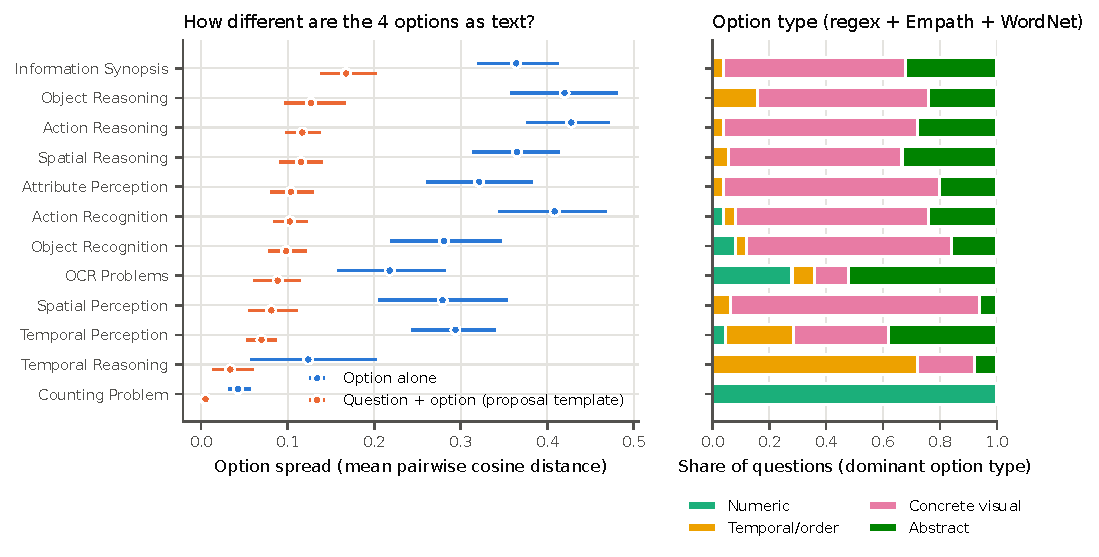
\includegraphics[width=\linewidth]{outputs/a1_language/fig1_option_spread.pdf}
  \caption{Sub-analysis 1. Left: option spread per task type (mean, 95\% bootstrap CI) for
  options alone vs.\ inside the proposal's question template. Right: dominant option type.}
  \label{fig:a1}
\end{figure}

\begin{figure}[t]
  \centering
  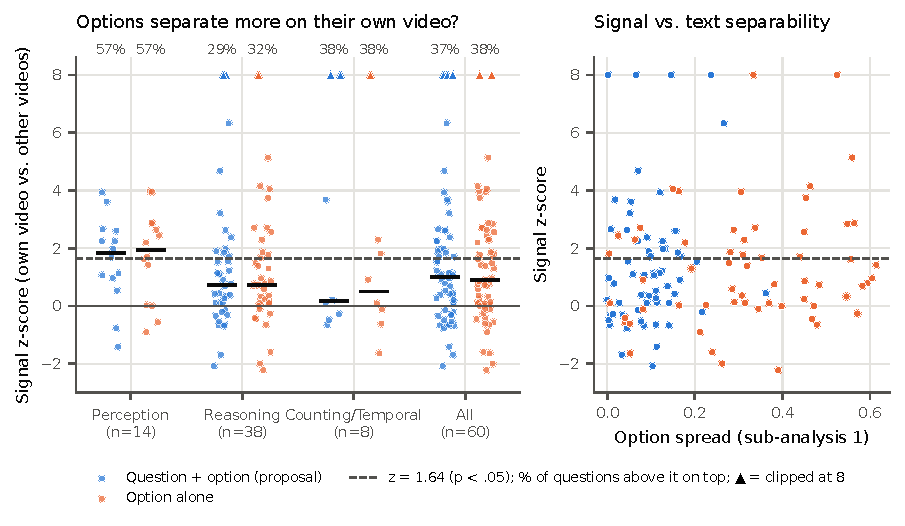
\includegraphics[width=\linewidth]{outputs/a2_signal/fig2_signal_vs_null.pdf}
  \caption{Sub-analysis 2. Left: per-question signal $z$-score (own video vs.\ 19 other
  videos); bars are medians, percentages are the share above $z{=}1.64$. Right: $z$ vs.\ option spread.}
  \label{fig:a2}
\end{figure}

\begin{figure}[t]
  \centering
  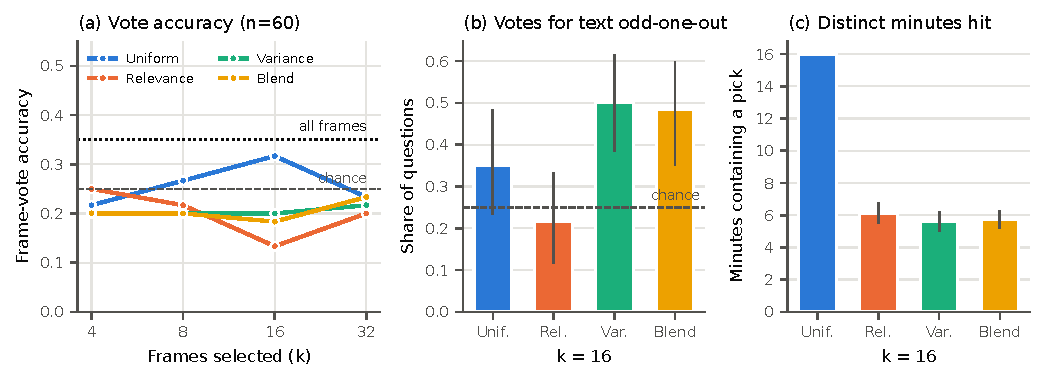
\includegraphics[width=\linewidth]{outputs/a3_task/fig3_frame_vote_opt_tmpl.pdf}
  \caption{Sub-analysis 3 (60 questions). (a) Frame-vote accuracy vs.\ budget $k$.
  (b) Share of questions whose top-16 vote goes to the textual odd-one-out option.
  (c) Distinct minutes containing a selected frame. Error bars: 95\% bootstrap CI.}
  \label{fig:a3}
\end{figure}

\begin{figure*}[t]
  \centering
  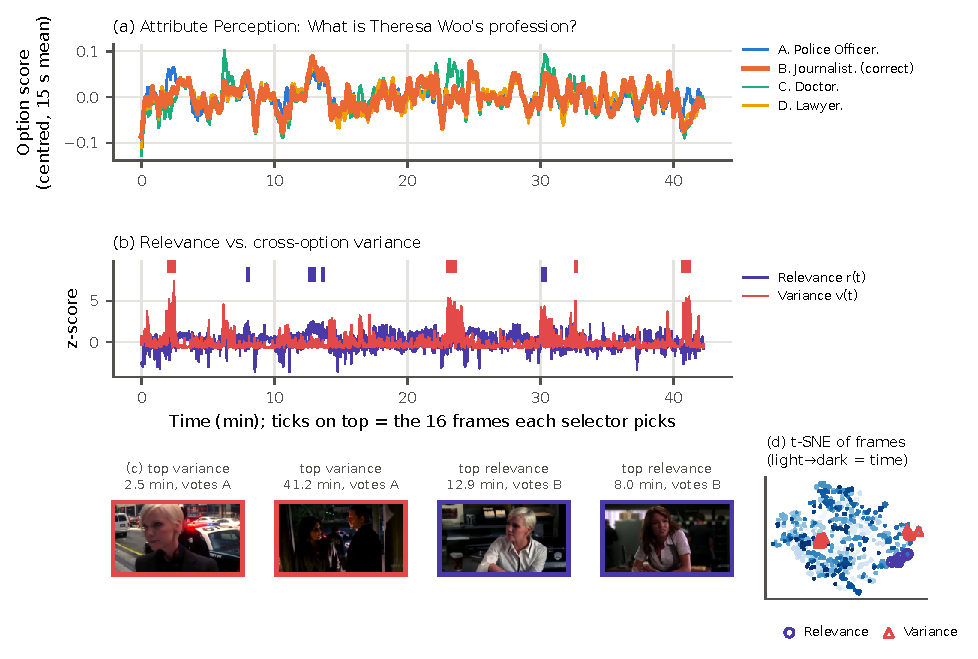
\includegraphics[width=0.85\textwidth]{outputs/a3_task/fig4_example_opt_tmpl.pdf}
  \caption{Example (Attribute Perception, 43-min video). (a) Centred option scores; (b)
  relevance and variance with each selector's 16 picks; (c) top frames: variance picks
  police-car scenes and votes for the distractor (A), while relevance picks the
  subject and votes for the answer (B); (d) t-SNE of all frames with the picks overlaid.}
  \label{fig:a4}
\end{figure*}
